\documentclass[border=10pt]{standalone} 
\usepackage{tikz}

\usetikzlibrary{calc}
\usetikzlibrary{arrows}
\usetikzlibrary{shadows}
\usetikzlibrary{patterns}
\usetikzlibrary{positioning}
\usetikzlibrary{shapes}
\usetikzlibrary{3d}
%\usetikzlibrary{automata}
\usetikzlibrary{fit}

\tikzset{block/.style={draw, text centered, fill=gray!10,drop shadow}}
\tikzset{connect/.style={draw, line width=1 pt}}

\begin{document}


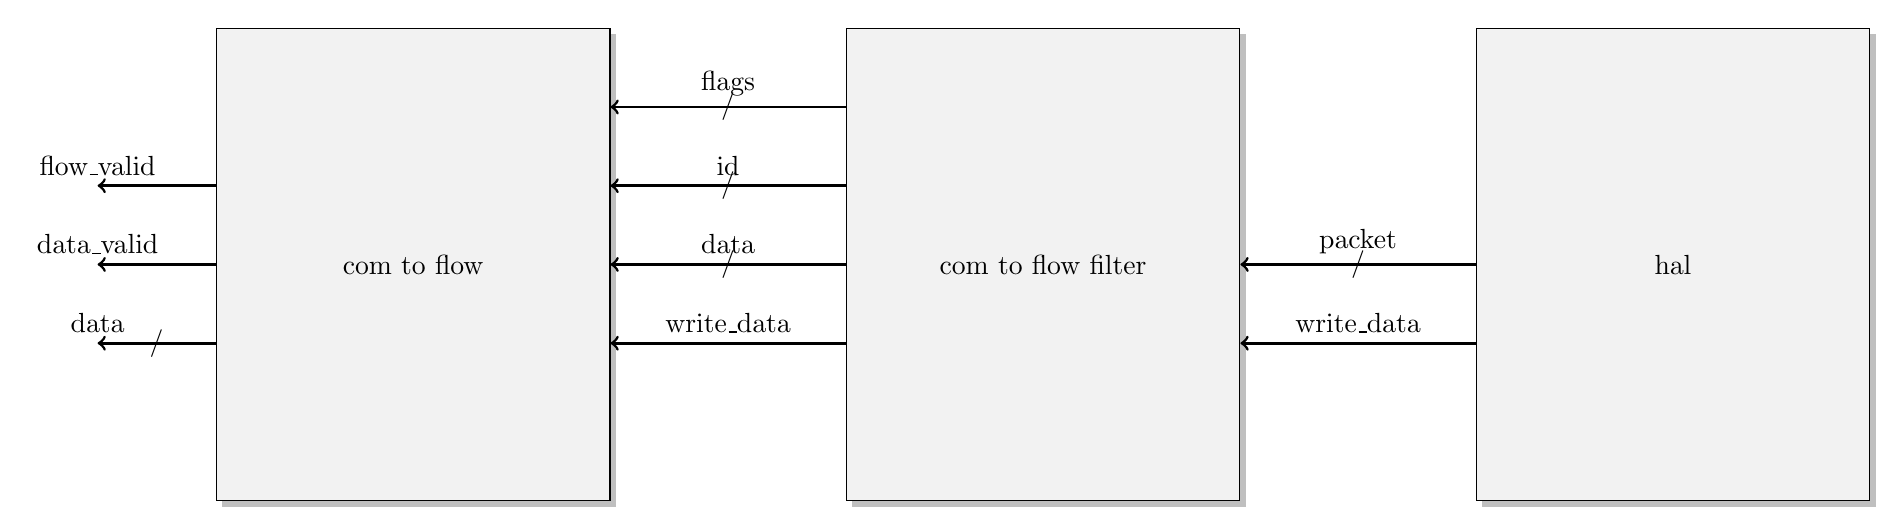
\begin{tikzpicture}

\node[block,minimum height=6cm,minimum width=5cm] (hal) {hal};
\node[block,minimum height=6cm,minimum width=5cm] (filter) at([xshift=-8cm]hal) {com to flow filter};
\node[block,minimum height=6cm,minimum width=5cm] (com) at([xshift=-8cm]filter) {com to flow};

\path[connect,<-] (filter.east) -- node{/} node[above]{packet} (hal.west);
\path[connect,<-] ([yshift=-1cm]filter.east) -- node[above]{write\_data} ([yshift=-1cm]hal.west);

\path[connect,<-] (com.east) -- node{/} node[above]{data} (filter.west);
\path[connect,<-] ([yshift=-1cm]com.east) --  node[above]{write\_data} ([yshift=-1cm]filter.west);
\path[connect,<-] ([yshift=1cm]com.east) -- node{/} node[above]{id} ([yshift=1cm]filter.west);
\path[connect,<-] ([yshift=2cm]com.east) -- node{/} node[above]{flags} ([yshift=2cm]filter.west);

\path[connect,->] ([yshift=-1cm]com.west) -- node{/} ++ (-1.5cm,0)  node[above]{data};
\path[connect,->] (com.west) -- ++ (-1.5cm,0)  node[above]{data\_valid};
\path[connect,->] ([yshift=1cm]com.west) -- ++ (-1.5cm,0)  node[above]{flow\_valid};




\end{tikzpicture}


\end{document}